\documentclass[problem]{mcs}

\begin{pcomments}
  \pcomment{from: S09.cp6r}
  \pcomment{from: S07.cp6m}
\end{pcomments}

\pkeywords{
  chromatic_number
  graph_coloring
}

%%%%%%%%%%%%%%%%%%%%%%%%%%%%%%%%%%%%%%%%%%%%%%%%%%%%%%%%%%%%%%%%%%%%%
% Problem starts here
%%%%%%%%%%%%%%%%%%%%%%%%%%%%%%%%%%%%%%%%%%%%%%%%%%%%%%%%%%%%%%%%%%%%%

\begin{problem}
Let $G$ be the graph below\footnote{From \emph{Discrete Mathematics},
Lov\'asz, Pelikan, and Vesztergombi. Springer, 2003.  Exercise 13.3.1}.
Carefully explain why $\chi(G)=4$.

\mfigure{!}{2in}{figures/4-chromatic}
\begin{solution}
Four colors are sufficient, so $\chi(G) \leq 4$.

\begin{figure}[h]\centering 
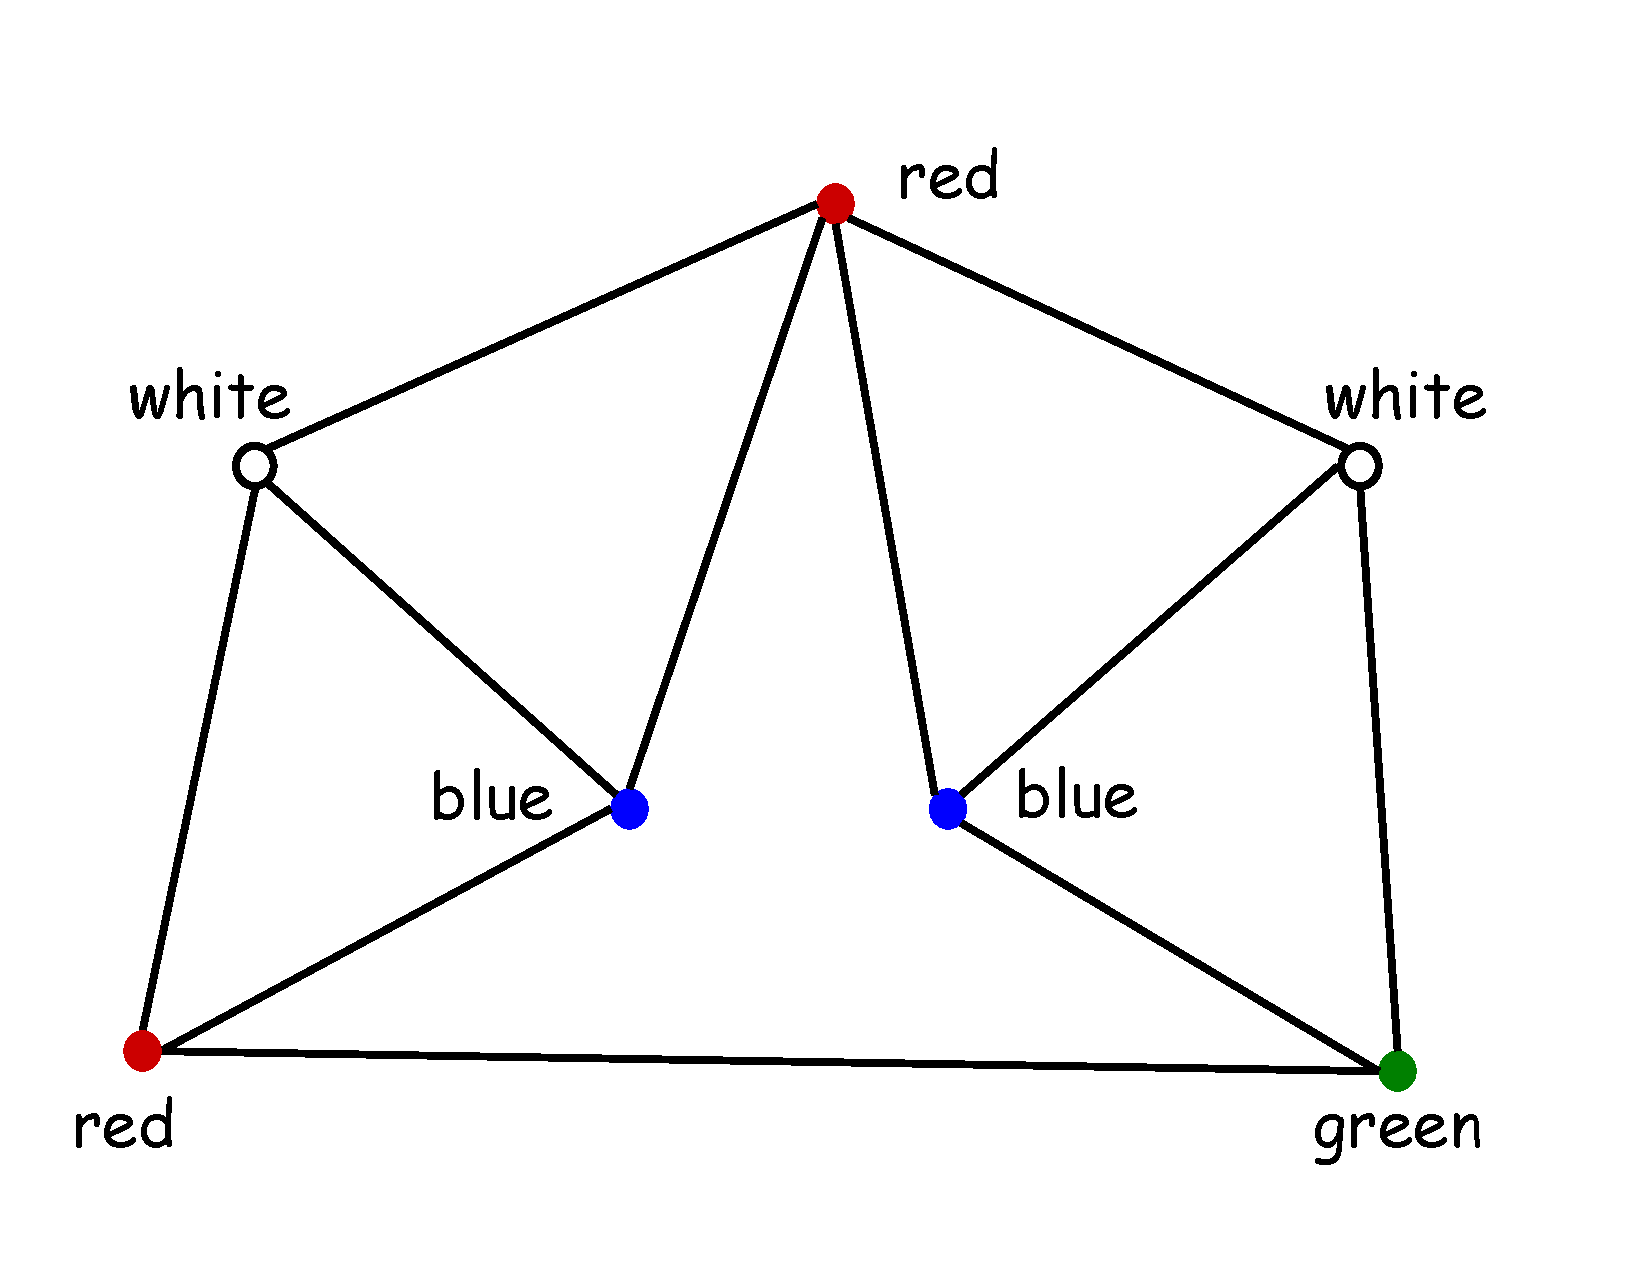
\includegraphics[height=2in]{figures/4-chromatic-colored}
\caption{A 4-coloring of the Graph}\label{fig:4-coloring}
\end{figure}

Now assume $\chi(G)=3$. We may assume the top vertex is colored red.  The
top two triangles require 3 colors each, and since they share the top red
vertex, they must have the other two colors, white and blue, at their
bases, as in Figure~\ref{fig:4-coloring}.  Now the bottom two vertices are
both adjacent to vertices colored white and blue, and cannot have the same
color since they are adjacent, so there is no alternative but to color one
with a third color and the other with a fourth color, contradicting the
assumption that 3 colors are enough.  Hence, $\chi(G)>3$.  This together
with~\eqref{chileq4} implies that $\chi(G)=4$.
\end{solution}

\end{problem}

%%%%%%%%%%%%%%%%%%%%%%%%%%%%%%%%%%%%%%%%%%%%%%%%%%%%%%%%%%%%%%%%%%%%%
% Problem ends here
%%%%%%%%%%%%%%%%%%%%%%%%%%%%%%%%%%%%%%%%%%%%%%%%%%%%%%%%%%%%%%%%%%%%%
